\documentclass[11pt]{beamer}
\usepackage[utf8]{inputenc}
\usepackage[spanish]{babel}
\usepackage{amsmath}
\usepackage{amsfonts}
\usepackage{amssymb}
\usepackage{graphicx}
\usepackage{lipsum}
\usepackage{ragged2e}
\usepackage{hyperref}
\usepackage{float}
\usepackage{url}
\usetheme{Madrid}
\newcommand{\celda}[1]{
	\begin{minipage}{2.5cm}
		\vspace{5mm}
		#1
		\vspace{5mm}
	\end{minipage}
}

\author[Laura]{Laura Carrasco Hernández\inst{1} \& Docentes-investigadores: Dr.Gonzalo Aranda - Dr. Adolfo Centeno  \inst{1}}
\title[Docking molecular]{Docking molecular de la proteína E del SARS-CoV-2 con la amantadina como ligando}
\date{8 de enero de 2020} 
\subtitle{Acoplamiento molecular con AutoDock Tools y AutoDock Vina}
\institute[UV]{
	\inst{1}
		Universidad Veracruzana. \\Instituto de Investigaciones Cerebrales.\\
		\vspace{2mm}
	
}

\AtBeginSection[]
{
	\begin{frame}<beamer>{Contenido}
		\tableofcontents[currentsection,currentsubsection]
	\end{frame}
}


\begin{document}
	
	\begin{frame}
		\maketitle
	\end{frame}

	\begin{frame}{Contenido}
		\tableofcontents
	\end{frame}

	\section{Resumen}
		\begin{frame}{Resumen}
			\justifying El SARS-Cov-2 es el virus de la nueva enfermedad COVID-19, la cual ha cobrado la vida de muchas personas en el mundo, sus síntomas incluyen tos, dolor de garganta, diarrea, insuficiencia respiratoria y temperatura. Se ha propuesto que la amantadina es un fármaco que disminuye los efectos del COVID- 19, por lo tanto, es importante demostrar mediante modelos de acoplamiento molecular cómo la amantadina actúa en este virus.
		\end{frame}
	
	\section{Introducción}
		\begin{frame}{Introducción}
			\justifying El virus del SARS-Cov-2 surgió en China en diciembre de 2019 y se propagó por todo el mundo con el nombre de COVID-19. 
			
			La envoltura del virus está formada por la proteína de envoltura o proteína E. está integrada por 75 aminoácidos, de los cuales se forma una estructura de hélice alfa de los aminoácidos 15 a 39 y los demás como estructuras secundarias en forma de espiral. Varias investigaciones demuestran que la carencia de proteína E mitiga el daño en los ratones que han sido infectados con COVID-19. Dentro de los estudios que se han mencionado, se destaca el uso de la Amantadina como posible atenuante de los efectos de COVID-19
			
			
			\end{frame}
			
			\begin{frame}{Introducción}
			Se sabe que cuando el virus ingresa a la célula, se crea un endosoma y el canal de protones que está formado por la proteína M2 transporta protones al interior del virión, lo cual, la amantadina atravieza el endosoma para interrumpir la liberación del virión a la célula. 
			
			Así mismo, la amantadina actúa e ingresa al canal E del SARS-Cov-2 y evita la liberación del virus en la célula. 
	Los estuidos de acoplamiento molecular de acuerdo a Aranda et al., (2020) han sugerido que la amantadina interactúa con varios aminoácidos del virus para bloquear el canal de protones.
		\end{frame}
		
	
	\section{Docking molecular}
		\begin{frame}{Docking molecular}
			\justifying El docking molecular o acoplamiento molecular, es un método bioinformático que permite descubrir y calcular la posición de interacción entre un ligando y un blanco proteico con una representación 3D.
			
			Para la realización del docking se utilizó el programa AutoDockTools-1.5.6 y AutoDock Vina, la proteína E del SARS-Cov-2, la Amantadina como ligando (DB00915) y los aminoácidos ASN15, LEU18 y LEU19
		\end{frame}
	
	\begin{frame}{Docking molecular}
			\justifying 
			a) Se inició con subir la proteína en formato .pdb al programa y representarla en cintas
			
			\begin{figure}[H]
				\centering
				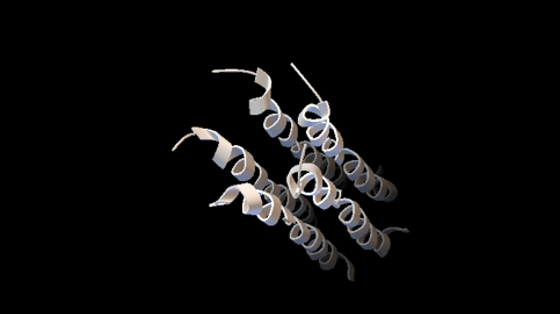
\includegraphics[scale=0.5]{Ecintas.png}
				\caption{Proteína E del SARS-CoV-2}
				\label{fig: Figura1}
			\end{figure}
		\end{frame} 
		
			\begin{frame}{Docking molecular}
			\justifying 
			b) Se integró la amantadina (DB00915) como archivo de ligando .pdb
			
			\begin{figure}[H]
				\centering
				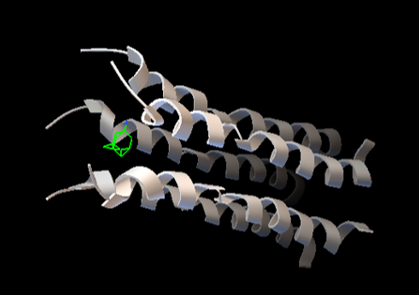
\includegraphics[scale=0.5]{Eyligando.png}
				\caption{Ligando: Amantadina (DB00915)}
				\label{fig: Figura1}
			\end{figure}
		\end{frame} 
			
			
				\begin{frame}{Docking molecular}
			\justifying 
			c) Se configuró el espacio de búsqueda con Grid Box para establecer la ubicación y la extensión del área 3D
			
			\begin{figure}[H]
				\centering
				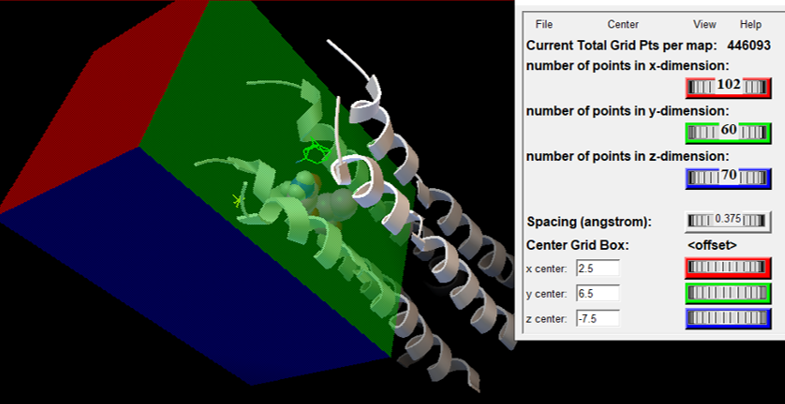
\includegraphics[scale=0.5]{grid.png}
				\caption{Ubicación y extensión del área 3D}
				\label{fig: Figura1}
			\end{figure}
		\end{frame} 
			
				\begin{frame}{Docking molecular}
			\justifying 
				d) Se hizo un acoplamiento corto con 250000 evaluaciones por correr y después se inició con AutoDock Vina. Se utilizó un CPU de 8, y una semilla aleatoria (random seed) de 200540960 
			
			\begin{figure}[H]
				\centering
				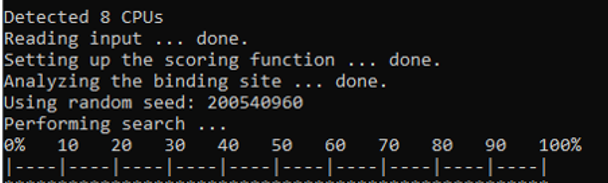
\includegraphics[scale=0.5]{semilla.png}
				\caption{Semilla aleatoria de docking}
				\label{fig: Figura1}
			\end{figure}
		\end{frame} 
			
				\begin{frame}{Docking molecular}
			\justifying 
				e) Se obtuvo la energía de afinidad en kcla/mol así como la desviación cuadrática media 
			
			\begin{figure}[H]
				\centering
				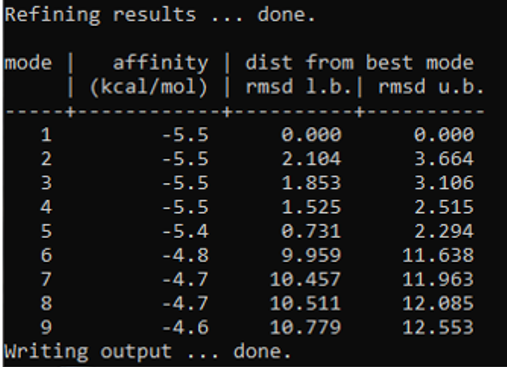
\includegraphics[scale=0.5]{afinidad.png}
				\caption{Energía de afinidad y desviación cuadrática}
				\label{fig: Figura1}
			\end{figure}
		\end{frame} 
			
			
				\begin{frame}{Docking molecular}
			\justifying 
				f) Con AutoDock Vina se utilizó una sola molécula de múltiples conformaciones, de los cuales se obtuvieron 9 conformaciones 
			
			\begin{figure}[H]
				\centering
				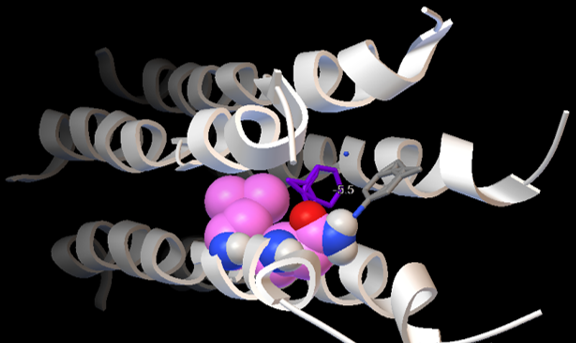
\includegraphics[scale=0.5]{conformaciones.png}
				\caption{Energía de afinidad principal}
				\label{fig: Figura1}
			\end{figure}
		\end{frame} 
			
			
			
				\begin{frame}{Docking molecular}
			\justifying 
				g) Por último se realizó el Docking mostrando las interacciones y la energía de afinidad 
			
			\begin{figure}[H]
				\centering
				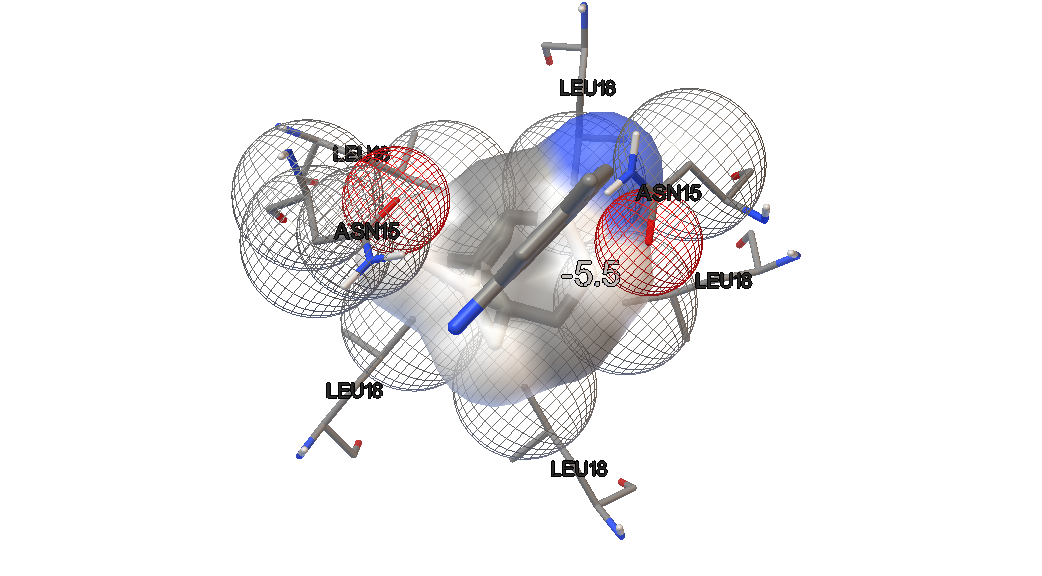
\includegraphics[scale=0.25]{Aminoacido y ligando.png}
				\caption{Docking con las interacciones}
				\label{fig: Figura1}
			\end{figure}
		\end{frame} 
		
			
			
				\begin{frame}{Docking molecular}
			\justifying 
				 h) También se muestran todos los residuos en la proteína para ubicar el sitio de interacción y unión
			
			\begin{figure}[H]
				\centering
				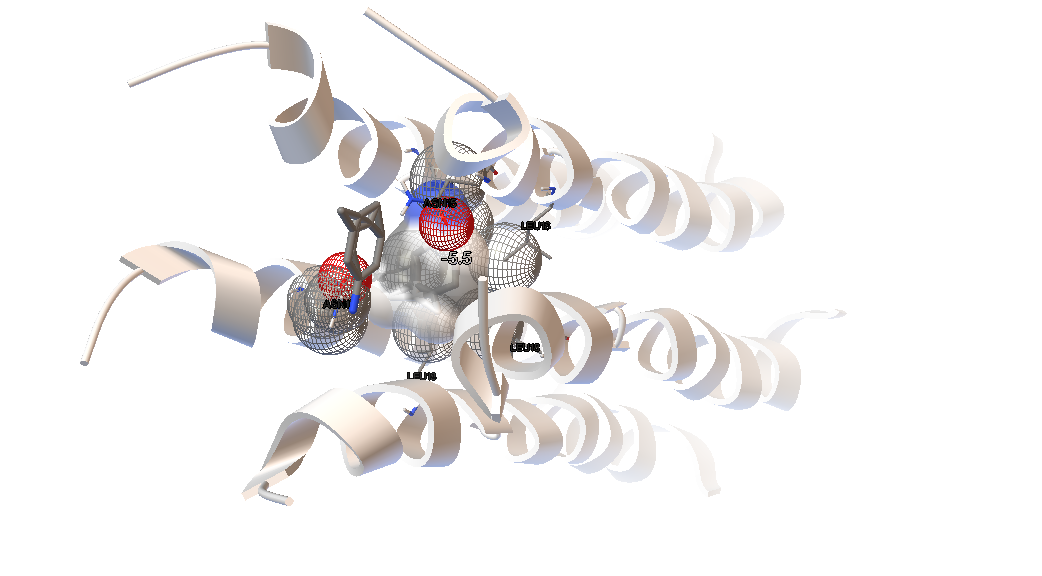
\includegraphics[scale=0.25]{Interaccion.png}
				\caption{Residuos en la proteína}
				\label{fig: Figura1}
			\end{figure}
		\end{frame} 
		
			

	
	\section{Conclusión}
		\begin{frame}{Conclusión}
			\justifying El docking molecular es un método que ayuda a conocer la unión más estable, específica y favorable entre un ligando y su blanco para contar con su actividad biológica y saber si es un ligando o fármaco efectivo.
Aranda, Hernández, Herrera y Rojas (2020) han propuesto un modelo describiendo a la amantadina como ligando que entra en el canal que se forma por la proteína E del virus para romper los puentes de hidrógeno formados con el agua como lo hace en la influenza A. Por lo que podría recomendarse a la amantadina para administrarse cuando se presentan los primeros síntomas de la enfermedad por COVID-19 y así atenuar los efectos del virus.
		\end{frame}
	
	

%\appendix
\section{Referencias}
%\subsection<presentation>*{Referencias}

\begin{frame}{Referencias}

\begin{thebibliography}{5}
	
	\beamertemplatearticlebibitems
	
	\bibitem{Aranda 2020}
Aranda, G., Hernández, M., Herrera, D. y Rojas, F. (2020). 
	\newblock{Amantadine as a drug to mitigate the effects of COVID-19. Medical Hypotheses, 140(April), 1–3. https://doi.org/10.1016/j.mehy.2020.109755}
	
	\bibitem{Araujo 2020}
	Araújo, R., Aranda, J. y Aranda, G. (2020).
	\newblock{ Amantadine Treatment for People with COVID-19. Archives of Medical Research. doi: 10.1016/j.arcmed.2020.06.009}
	
	\bibitem{Ballon 2019}
	Ballón, W. y Grados, R. (2019). 
	\newblock{Acomplamiento molecular: criterios prácticos para la selección de ligandos biológicamente activos e identificación de nuevos blancos terapéuticos. Revista Con-Ciencia. 2(7): 55-72.}

	\bibitem{Huey 2012}
	Huey, R., Morris, G. y Forli, S. (2012). 
	\newblock{Using AutoDock4 and AutoDock Vina with AutoDockTools: A tutorial. USA: The Scripps Research Institute}
	
\end{thebibliography}
\end{frame}
\end{document}